%% ============================================================
%%  Presentación – Proyecto Grupo-2
%%  UK Road Safety: Traffic Accidents and Vehicles (2010–2017)
%%  Estilo: Geométrico / Editorial
%%  Compilar: pdflatex → biber → pdflatex × 2
%% ============================================================

\documentclass[aspectratio=169, 10pt]{beamer}

\usepackage[utf8]{inputenc}
\usepackage[T1]{fontenc}
\usepackage[spanish]{babel}
\usepackage{csquotes}
\usepackage{lmodern}
\usepackage{microtype}
\usepackage{graphicx}
\usepackage{tikz}
\usetikzlibrary{calc}
\usepackage{booktabs}
\usepackage{amsmath, amssymb}
\usepackage{xcolor}
\usepackage{tcolorbox}
\tcbuselibrary{skins, breakable}
\usepackage[backend=biber, style=apa, sorting=nyt]{biblatex}
\addbibresource{../referencias/referencias.bib}

%% ── Colores ─────────────────────────────────────────────────
\definecolor{Verde}{HTML}{1F4E3D}
\definecolor{VerdeM}{HTML}{2D6A4F}
\definecolor{VerdeC}{HTML}{74C69D}
\definecolor{Naranja}{HTML}{C96A1E}
\definecolor{NaranjaC}{HTML}{E8914A}
\definecolor{Crema}{HTML}{FCFAF7}
\definecolor{GrisO}{HTML}{3A3A3A}
\definecolor{GrisC}{HTML}{888888}

%% ── Tema limpio ──────────────────────────────────────────────
\usetheme{default}
\usecolortheme{default}
\usefonttheme{professionalfonts}
\setbeamertemplate{navigation symbols}{}
\setbeamertemplate{frametitle}{}
\setbeamertemplate{footline}{}
\setbeamertemplate{headline}{}
\setbeamercolor{background canvas}{bg=Crema}
\setbeamercolor{normal text}{fg=GrisO}
\setbeamercolor{itemize item}{fg=Naranja}
\setbeamercolor{itemize subitem}{fg=VerdeC}
\setbeamertemplate{itemize item}{\small\raisebox{1pt}{$\blacktriangleright$}}
\setbeamertemplate{itemize subitem}{\small$\circ$}

%% ── Cabecera (sin texto con acentos dentro de TikZ) ─────────
\newcommand{\frameheader}[2]{%
  \begin{tikzpicture}[remember picture, overlay]
    \fill[Verde] (current page.north west)
      rectangle ([yshift=-1.15cm] current page.north east);
    \fill[Naranja] (current page.north west)
      rectangle ([xshift=0.45cm, yshift=-1.15cm] current page.north west);
    \fill[NaranjaC] ([xshift=-0.35cm] current page.north east)
      rectangle ([xshift=0cm, yshift=-1.15cm] current page.north east);
  \end{tikzpicture}%
  % Texto fuera de TikZ, posicionado con \makebox
  \begin{tikzpicture}[remember picture, overlay]
    \node[anchor=west, text=VerdeC, font=\tiny\bfseries]
      at ([xshift=0.65cm, yshift=-0.38cm] current page.north west)
      {\MakeUppercase{#1}};
    \node[anchor=west, text=white, font=\normalsize\bfseries]
      at ([xshift=0.65cm, yshift=-0.80cm] current page.north west)
      {#2};
  \end{tikzpicture}%
  \vspace{0.78cm}%
}

%% ── Pie de página ────────────────────────────────────────────
\newcommand{\myfooter}{%
  \begin{tikzpicture}[remember picture, overlay]
    \fill[Verde!90] (current page.south west)
      rectangle ([yshift=0.45cm] current page.south east);
    \fill[Naranja]
      ([xshift=-0.8cm] current page.south east)
      rectangle
      ([yshift=0.45cm] current page.south east);
  \end{tikzpicture}%
  \begin{tikzpicture}[remember picture, overlay]
    \node[anchor=west, text=VerdeC!70!white, font=\tiny]
      at ([xshift=0.3cm, yshift=0.22cm] current page.south west)
      {Grupo 2 \textperiodcentered{} CA0303 \textperiodcentered{} UCR};
    \node[anchor=east, text=white, font=\tiny\bfseries]
      at ([xshift=-1.0cm, yshift=0.22cm] current page.south east)
      {\insertframenumber/\inserttotalframenumber};
  \end{tikzpicture}%
}

%% ── Cajas tcolorbox ──────────────────────────────────────────
\tcbset{
  bloqueverde/.style={
    enhanced, boxrule=0pt, arc=3pt,
    colback=Verde!8, colframe=Verde, leftrule=4pt,
    top=8pt, bottom=6pt,
    fonttitle=\small\bfseries, coltitle=white,
    attach boxed title to top left={yshift=-2mm, xshift=4mm},
    boxed title style={colback=Verde, arc=2pt, boxrule=0pt}
  },
  bloquenaranja/.style={
    enhanced, boxrule=0pt, arc=3pt,
    colback=Naranja!8, colframe=Naranja, leftrule=4pt,
    top=8pt, bottom=6pt,
    fonttitle=\small\bfseries, coltitle=white,
    attach boxed title to top left={yshift=-2mm, xshift=4mm},
    boxed title style={colback=Naranja, arc=2pt, boxrule=0pt}
  },
  bloquementa/.style={
    enhanced, boxrule=0pt, arc=3pt,
    colback=VerdeC!15, colframe=VerdeC!60!Verde, leftrule=4pt,
    top=8pt, bottom=6pt,
    fonttitle=\small\bfseries, coltitle=white,
    attach boxed title to top left={yshift=-2mm, xshift=4mm},
    boxed title style={colback=VerdeC!60!Verde, arc=2pt, boxrule=0pt}
  }
}

%% ── Nodo de dato destacado ───────────────────────────────────
\newcommand{\datobig}[2]{%
  \begin{tikzpicture}
    \fill[Verde] (0,0) rectangle (2.8cm, 1.4cm);
    \fill[Naranja] (0,0) rectangle (0.15cm, 1.4cm);
  \end{tikzpicture}%
  % Superposición del texto con llapbox
  \llap{%
    \begin{minipage}[b][1.4cm][c]{2.8cm}
      \centering
      {\color{white}\large\bfseries #1}\\[-2pt]
      {\color{VerdeC}\tiny #2}
    \end{minipage}%
  }%
}

%% ── Bloque de color decorativo (sin texto) ───────────────────
\newcommand{\geoblocks}{%
  \begin{tikzpicture}
    \fill[Verde!15]   (0,0)    rectangle (3cm, 3.5cm);
    \fill[Naranja!25] (0.15cm,0.15cm) rectangle (1.2cm,1.2cm);
    \fill[VerdeC!35]  (1.4cm,2.1cm)   rectangle (2.9cm,3.3cm);
    \fill[Verde!40]   (0.15cm,1.4cm)  rectangle (0.9cm,2.0cm);
    \fill[NaranjaC!20](1.4cm,0.2cm)   rectangle (2.85cm,1.85cm);
  \end{tikzpicture}%
}

%% ============================================================
\begin{document}
%% ============================================================

%% ── PORTADA ──────────────────────────────────────────────────
\setbeamercolor{background canvas}{bg=Verde}
\begin{frame}[plain]
  \begin{tikzpicture}[remember picture, overlay]
    % Bloque naranja derecho
    \fill[Naranja]
      ([xshift=-4.2cm] current page.north east)
      rectangle (current page.south east);
    % Triángulo VerdeM
    \fill[VerdeM]
      ([xshift=-4.2cm] current page.north east) --
      ([xshift=-4.2cm, yshift=-3.5cm] current page.north east) --
      ([xshift=-7.5cm] current page.north east) -- cycle;
    % Rectángulo pequeño NaranjaC
    \fill[NaranjaC!60]
      ([xshift=-4.2cm, yshift=-3.5cm] current page.north east)
      rectangle ([xshift=-3.0cm, yshift=-4.1cm] current page.north east);
    % Línea VerdeC
    \draw[VerdeC, line width=1.2pt]
      ([xshift=1.2cm,  yshift=-4.8cm] current page.north west) --
      ([xshift=-4.5cm, yshift=-4.8cm] current page.north east);
  \end{tikzpicture}%
  % Texto de portada fuera de TikZ geométrico
  \begin{tikzpicture}[remember picture, overlay]
    \node[anchor=west, text=VerdeC, font=\tiny\bfseries, text width=9cm]
      at ([xshift=1.2cm, yshift=-2.0cm] current page.north west)
      {CA0303 \textperiodcentered{} ESTAD\'ISTICA ACTUARIAL I \textperiodcentered{} GRUPO 2};
    \node[anchor=west, text=white, font=\LARGE\bfseries, text width=10cm]
      at ([xshift=1.2cm, yshift=-3.5cm] current page.north west)
      {Factores relacionados a accidentes\\de tr\'ansito en el\\Reino Unido (2010-2017)};
    
      \node[anchor=west, text=VerdeC!80!white, font=\small, text width=9cm]
      at ([xshift=1.2cm, yshift=-5.8cm] current page.north west)
      {Debbie Con Ortega     C32250 \\
       Ashly Garro           C33198\\
       Emily Sanchéz Mancía  C27260\\
       Alessandro Umaña Vega C37963};
    \node[anchor=west, text=NaranjaC, font=\normalsize\bfseries]
      at ([xshift=1.2cm, yshift=-6.1cm] current page.north west)
      {};
    \node[anchor=center, text=white, font=\small\bfseries,
          text width=3.8cm, align=center]
      at ([xshift=-2.1cm, yshift=-5.5cm] current page.north east)
      {Universidad de Costa Rica };
  \end{tikzpicture}
\end{frame}
\setbeamercolor{background canvas}{bg=Crema}

%% ── CONTENIDO ────────────────────────────────────────────────
\begin{frame}[plain]
  \frameheader{}{Contenido}
  \myfooter
  \vspace{0.4cm}
  \begin{columns}[T]

    \begin{column}{0.50\textwidth}
      \renewcommand{\arraystretch}{1.6}
      \begin{tabular}{@{}c l l@{}}
        
        \textcolor{Verde}{\rule{7pt}{16pt}} &
        \textbf{1.} & \large Pregunta de Investigaci\'on\\

        \textcolor{VerdeM}{\rule{7pt}{16pt}} &
        \textbf{2.} & \large Datos\\

        \textcolor{VerdeM}{\rule{7pt}{16pt}} &
        \textbf{3.} & \large Metodolog\'ia Propuesta\\

        \textcolor{Naranja}{\rule{7pt}{16pt}} &
        \textbf{4.} & \large Resultados Esperados \\
      \end{tabular}

    \end{column}

    \begin{column}{0.42\textwidth}
      \centering
    \end{column}

  \end{columns}

\end{frame}

%% ============================================================
\section{Pregunta de Investigaci\'on}
%% ============================================================

\begin{frame}[plain]
  \frameheader{01}{Pregunta de Investigaci\'on}
  \myfooter
  \begin{columns}[T]
    \begin{column}{0.60\textwidth}
      \begin{tcolorbox}[bloqueverde, title=Pregunta central]
        \small
        ¿Cómo varía la cantidad de accidentes de tránsito en el
        Reino Unido en función de distintos factores del entorno durante el periodo
        \textbf{2010--2017}?\\[6pt]
        Se utilizará la base de datos \textbf{UK Road Safety: Traffic
        Accidents and Vehicles} con el objetivo de
        \textbf{identificar situaciones de riesgo} y proponer
        \textbf{medidas de prevención} que contribuyan a reducir la
        frecuencia de accidentes.
      \end{tcolorbox}
    \end{column}

    \begin{column}{0.36\textwidth}
      \begin{tcolorbox}[bloquenaranja, title=Audiencia objetivo]
        \small 
        Investigadores académicos en:
        \begin{itemize}
          \item Estadística
          \item Análisis de datos
          \item Seguridad vial
        \end{itemize}
      \end{tcolorbox}
    \end{column}

  \end{columns}
\end{frame}

%% ============================================================
\section{Datos}
%% ============================================================

\begin{frame}[plain]
  \frameheader{02}{Datos -- Fuente y Variables}
  \myfooter
  \begin{columns}[T]
    \begin{column}{0.46\textwidth}
      \begin{tcolorbox}[bloqueverde, title=Fuente de datos]
        \small
        \text{UK Road Safety Accidents and Vehicles}\\[3pt]
        {\color{GrisC}\footnotesize Kaggle-Departamento de Transporte del Reino Unido}
      \end{tcolorbox}
      \vspace{8pt}
    \end{column}
    \begin{column}{0.50\textwidth}
      \begin{tcolorbox}[bloqueverde, title=Descripción de los datos]
        \begin{itemize}\small
          \item + 30  variables disponibles 
          \item 2,047,256 observaciones de accidentes 
          \item Período de observaciones: 2005-2017 
        \end{itemize}
      \end{tcolorbox}
    \end{column}
  \end{columns}

  \begin{tcolorbox}[bloquenaranja, title=Limitaciones]
    \begin{itemize}
      \item Diferencias regionales y restricciones de privacidad pueden afectar la consistencia de la recolección de datos.
      \item Datos faltantes y posibles sesgos en variables pueden reducir la precisión del análisis.
      \item Cambios en políticas, infraestructura y normativas a lo largo del tiempo pueden influir en los resultados sin reflejarse directamente en la base de datos.
    \end{itemize}
  \end{tcolorbox}
\end{frame}

%% ── Gráficos (2×2) ───────────────────────────────────────────
\begin{frame}[plain]
  \frameheader{02}{Datos -- Resultados Exploratorios}
  \myfooter
  \begin{columns}[T]
    \begin{column}{0.5\textwidth}
      \textbf{Condición climática}\\[2pt]
      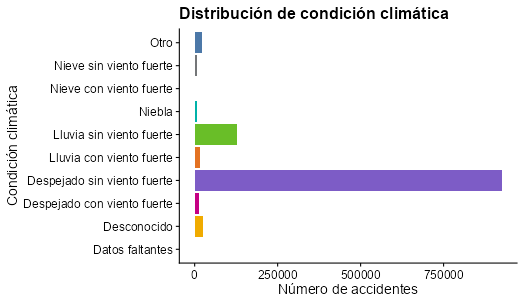
\includegraphics[width=\textwidth]{../bitacoras/bitacora_2/figuras/Distribucion_clima.png}
    \end{column}

    \begin{column}{0.5\textwidth}
      \textbf{Obstáculos en intersecciones T}\\[2pt]
      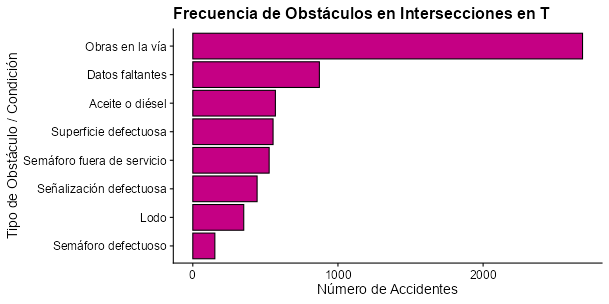
\includegraphics[width=\textwidth]{../bitacoras/bitacora_2/figuras/Frecuencia_Obstáculos_Intersecciones_T.png}
    \end{column}
  \end{columns}
\end{frame}

\begin{frame}[plain]
  \frameheader{02}{Datos -- Resultados Exploratorios}\\[2pt]
  \myfooter
  \textbf{Superficie de la vía y condición de luz}
  \centering
  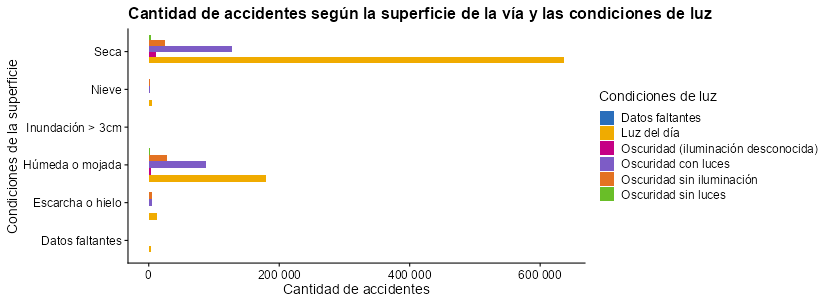
\includegraphics[width=0.7\textwidth]{../bitacoras/bitacora_2/figuras/Accidentes_superficiexluz.png}
\end{frame}

\begin{frame}
  \myfooter
   \frameheader{02}{Datos -- Resultados Exploratorios}\\[1.8pt]
  \textbf{Condición de carretera}

  \centering
  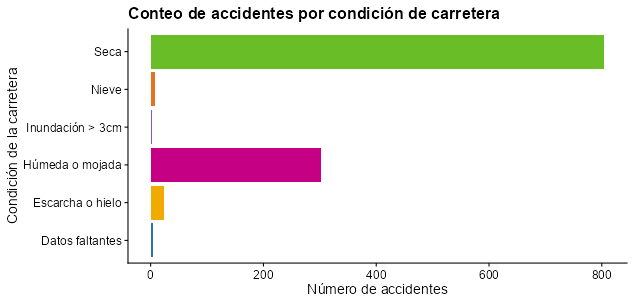
\includegraphics[width=0.65\textwidth]{../bitacoras/bitacora_2/figuras/frecuencia_condicion_calle.png}
\end{frame}

%% ============================================================
\section{Metodolog\'ia Propuesta}
%% ============================================================

\begin{frame}[plain]
  \frameheader{03}{Metodología propuesta}
  \myfooter
  \begin{columns}[T]
    \begin{column}{0.65\textwidth}
      \begin{tcolorbox}[bloqueverde, title=Tablas de contingencia]
        \small
        Tabla de distribución de frecuencias conjuntas de dos variables aleatorias clasificadas en categorías (\cite{LASTRE2019})
      \end{tcolorbox}

      \begin{tcolorbox}[bloqueverde, title=Pruebas de independencia $\chi^2$]
        \small
        Permite determinar si dos variables categóricas están relacionadas significativamente (\cite{LASTRE2019})
      \end{tcolorbox}

      \begin{tcolorbox}[bloqueverde, title=Pruebas de homogeneidad $\chi^2$]
        \small
        Determina si las proporciones de una variable categórica se mantienen constantes entre distintas
        categorías o si existen diferencias significativas (\cite{MONTANA2025})
      \end{tcolorbox}
    \end{column}

    \begin{column}{0.34\textwidth}
      \begin{tcolorbox}[bloquenaranja, title=Alternativas descartadas]
        \small\textbf{Distribución de Poisson:}\\
        {\footnotesize\color{GrisC}
          Orientada a modelos predictivos de conteo;
          no al análisis de relaciones.}

        \vspace{5pt}
        \small\textbf{Binomial Negativa:}\\
        {\footnotesize\color{GrisC}
          Misma razón: el enfoque es inferencial,
          no predictivo.}
      \end{tcolorbox}
    \end{column}
  \end{columns}
\end{frame}

%% ============================================================
\section{Resultados Esperados}
%% ============================================================

\begin{frame}[plain]
  \frameheader{04}{Resultados Esperados}
  \myfooter
  \begin{columns}[T]
    \begin{column}{0.48\textwidth}
      \begin{tcolorbox}[bloqueverde, title={¿Qué se espera obtener?}]
        \begin{itemize}\small
          \item Identificar cuáles variables tienen una relación significativa con la frecuencia
           de los accidentes de tránsito.
          \item Determinar qué factores presentan mayor incidencia (por ejemplo, intersecciones, obstáculos en vía, día de la semana).
          \item Generar hallazgos útiles para futuras regulaciones, recomendaciones viales y estudios replicables en otros contextos.
        \end{itemize}
      \end{tcolorbox}
    \end{column}
    \begin{column}{0.48\textwidth}
      \begin{tcolorbox}[bloquementa, title=Criterios de respuesta]
        \small ¿Cómo saber si se respondió la pregunta?
        \begin{itemize}\small
          \item Se identifican relaciones claras o ausencia de relación entre las variables analizadas y la frecuencia de accidentes.
          \item Las pruebas estadísticas permiten confirmar o rechazar las hipótesis planteadas sobre factores de riesgo.
          \item Los resultados ofrecen conclusiones aplicables para recomendaciones, regulación vial o futuras investigaciones.
        \end{itemize}
      \end{tcolorbox}
    \end{column}
  \end{columns}
\end{frame}

%% ── REFERENCIAS ──────────────────────────────────────────────
\begin{frame}[plain, allowframebreaks]
  \frameheader{}{Referencias}
  \myfooter
  \printbibliography[heading=none]
\end{frame}

%% ── CIERRE ───────────────────────────────────────────────────
\setbeamercolor{background canvas}{bg=Verde}
\begin{frame}[plain]
  \begin{tikzpicture}[remember picture, overlay]
    \fill[Naranja]
      ([xshift=-3.5cm] current page.north east)
      rectangle (current page.south east);
    
    \draw[VerdeC, line width=1pt]
      ([xshift=-6.5cm, yshift=-0.3cm] current page.center) --
      ([xshift=0.4cm,  yshift=-0.3cm] current page.center);
  \end{tikzpicture}
  \begin{tikzpicture}[remember picture, overlay]
    \node[text=white, font=\Huge\bfseries, anchor=center]
      at ([xshift=-3cm, yshift=1.0cm] current page.center)
      {¡Gracias!};
    \node[text=VerdeC, font=\small, anchor=center]
      at ([xshift=-3cm, yshift=0.1cm] current page.center)
      {Grupo 2 \textperiodcentered{} CA0303 \textperiodcentered{} UCR};
    \node[text=white, font=\small\bfseries, align=center, anchor=center]
      at ([xshift=-1.75cm] current page.east |- current page.center)
      {Escuela de\\Matem\'atica\\UCR};
  \end{tikzpicture}
\end{frame}

\end{document}